\subsection{Influence}

Let us now define the notions of influence between rules, that allows us to overapproximate the relations of causality and inhibition between events.

\begin{definition}[Multisum]
  Let $G_1$ and $G_2$ be two graphs. The \emph{multisums} of $G_1$ and $G_2$ is a family of cospans of monos $G_1\lemb M_i\remb G_2$ such that for any other cospan of monos $G_1\lemb M'\remb G_2$ there exists a unique $M_k$, $k\leq n$ and a unique mono $M_k\lemb M'$:
  \[
  \begin{tikzpicture} %[scale=0.8]
    \node (l1) at (-1.5,0) {\(G_1\)};
    \node (l2) at (1.5,0) {\(G_2\)};
    \node (m1) at (-1,1) {\(M_1\)};
    \node (m2) at (0,1) {\(\cdots\)};
    \node (mn) at (1,1) {\(M_n\)};
    \node (n) at (0,2.5) {\(M'\)};
    \draw [right hook->] (l1) -- (m1);
    \draw [left hook->] (l2) -- (m1);
    \draw [right hook->] (l1) -- (mn);
    \draw [left hook->] (l2) -- (mn);
    \draw [right hook->] (l1) to [bend left] (n);
    \draw [left hook->] (l2) to [bend right] (n);
    \draw [left hook->, dotted] (m1) -- (n);
  \end{tikzpicture}
  \]
\end{definition}

\begin{remark}
  In using monos in the definition above, we define a family of cospans instead of defining the sum or disjoint union of $G_1$ and $G_2$.
\end{remark}

\begin{definition}[Pullback]
  The \emph{pullback} of the cospan $G_1\rightarrow M\leftarrow G_2$ is the span $G_1\leftarrow O\rightarrow G_2$ such that the following diagram commutes
  \[
  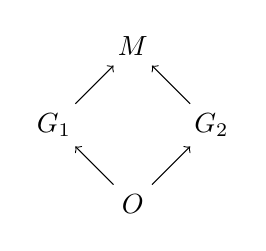
\begin{tikzpicture} %[scale=0.8]
    \node (o) at (0,-1) {\(O\)};
    \node (l1) at (-1,0) {\(G_1\)};
    \node (l2) at (1,0) {\(G_2\)};
    \node (m) at (0,1) {\(M\)};
    \draw [->] (o) --  (l1);
    \draw [->] (o) --  (l2);
    \draw [->] (l1) --  (m);
    \draw [->] (l2) --  (m);
  \end{tikzpicture}
  \]
  and such that for any other span $G_1\leftarrow O'\rightarrow G_2$ for which the diagram commutes, there is a unique morphism $O'\to O$:
  \[
  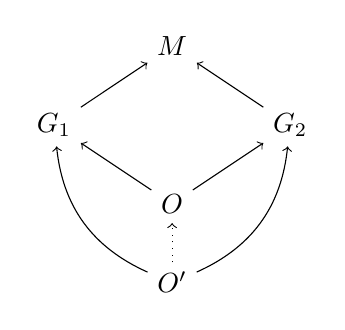
\begin{tikzpicture} %[scale=0.8]
    \node (o) at (0,-1) {\(O\)};
    \node (l1) at (-1.5,0) {\(G_1\)};
    \node (l2) at (1.5,0) {\(G_2\)};
    \node (m) at (0,1) {\(M\)};
    \node (n) at (0,-2) {\(O'\)};
    \draw [->] (o) --  (l1);
    \draw [->] (o) --  (l2);
    \draw [->] (l1) --  (m);
    \draw [->] (l2) --  (m);
    \draw [->] (n) to [bend left] (l1);
    \draw [->] (n) to [bend right] (l2);
    \draw [->, dotted] (n) -- (o);
  \end{tikzpicture}
  \]
\end{definition}

\begin{property}
  \begin{itemize}
  \item The pullback is unique up to isomorphism.
  \item The pullback preserves monos: if $G_i\to M$ is a mono then $O\to G_i$ is also a mono.
  \end{itemize}
\end{property}

\begin{definition}[Positive influence]
  \label{def:low_res}
  Let $L_1{\remb} D_1 {\lemb} R_1$ and $L_2{\remb} D_2 {\lemb} R_2$ be two rules.

  Let the cospan $R_1\lemb M\remb L_2$ be in the multisum of $R_1$ and $L_2$, from which we get the span $R_1\leftarrow O\rightarrow L_2$ as pullback.

  There is a \emph{positive influence} between the two rules induced by $O$ and denoted $r_1\redl{+}_o r_2$ if the pullback of the cospan $D_1\lemb R_1\remb O$, denoted $P$, and $O$ is not an iso. In other words, $O$ is not contained in $P$.
  \[
  \begin{tikzpicture} %[scale=0.8]
    \node (p) at (0,-1) {\(P\)};
    \node (d1) at (-1,0) {\(D_1\)};
    \node (o) at (1,0) {\(O\)};
    \node (m) at (1,2) {\(M\)};
    \node (r1) at (0,1) {\(R_1\)};
    \node (l1) at (-2,1) {\(L_1\)};
    \node (l2) at (2,1) {\(L_2\)};
    \draw [right hook->] (p) -- (d1);
    \draw [left hook->] (p) -- node [right,midway] {$\not\iso$}  (o);
    \draw [right hook->] (d1) -- (r1);
    \draw [right hook->] (d1) -- (l1);
    \draw [left hook->] (o) -- (r1);
    \draw [left hook->] (o) -- (l2);
    \draw [left hook->] (r1) --  (m);
    \draw [left hook->] (l2) --  (m);
  \end{tikzpicture}
  \]

  Define $r_1\redl{+} r_2$ if there exists $O$ such that $r_1\redl{+}_o r_2$.
\end{definition}

Similarly, define the negative influence $r_1\redl{-}_O r_2$ if there exists the span $L_1{\remb} O {\lemb} L_2$ and there is no iso between the pullback of the cospan $D_1\lemb L_1\remb O$ and $O$.

\begin{remark}[Influence in Kappa]
  In categories where the multisum between two graphs can be empty (such as the category of site graphs in Kappa), we can distinguish between \emph{low resolution} ifluence, in case the multisum is empty, and \emph{medium resolution} otherwise. There is a third notion of \emph{high resolution} influence which additionally checks that the graph $M$ of the multisum cospans, is reachable from an initial graph.
\end{remark}

\begin{lemma}
\label{lemma:pos_infl}
  $e< e'\implies \labl(e)\xrightarrow{+}\labl(e')$.
\end{lemma}
\begin{proof}
  \begin{mdframed}[backgroundcolor=blue!20]
    to do
  \end{mdframed}
\end{proof}

\begin{lemma}
  $e\dashv e' \implies\labl(e)\xrightarrow{-}\labl(e')$.
\end{lemma}
\begin{proof}
  \begin{mdframed}[backgroundcolor=blue!20]
    to do
  \end{mdframed}
\end{proof}

\begin{remark}[Influence and posets in Kappa]
  \autoref{lemma:pos_infl} is reformulated in site graphs as follows:
  \[e< e'\implies \labl(e)\xrightarrow[low]{+}\labl(e').\]
%% Note that if $e_1\ll e_2$ there are three cases possible:
%% \begin{itemize}
%% \item $e_1< e_2$
%% \item $\labl(e)\xrightarrow{+}\labl(e')$ and $\neg(e_1 < e_2)$
%% \item $\neg(\labl(e)\xrightarrow{+}\labl(e'))$
%% \end{itemize}
\end{remark}
